\documentclass[en]{../../../eplsummary}

\hypertitle{cloud-INGI2145}{7}{INGI}{2145}
{Houtain Nicolas, Thibault Gérondal}
{Canini Marco}

\section{Introduction}


\section{Summary of Eventually Consistent}

Data inconsistency in large-scale reliable distributed systems has to be tolerated for two reasons: improving read and write performance under highly concurrent conditions; and handling partition cases where a majority model would render part of the system unavailable even though the nodes are up and running.

Whether or not inconsistencies are acceptable depends on the client application. In all cases the developer needs to be aware that consistency guarantees are provided by the storage systems and need to be taken into account when developing applications.

\begin{description}
\item[Strong consistency] After the update completes, any subsequent access (by A, B, or C) will return the updated value.

\item[Weak consistency] The system does not guarantee that subsequent accesses will return the updated value. A number of conditions need to be met before the value will be returned. The period between the update and the moment when it is guaranteed that any observer will always see the updated value is dubbed the inconsistency window.

\item[Eventual consistency] This is a specific form of weak consistency; the storage system guarantees that if no new updates are made to the object, eventually all accesses will return the last updated value. If no failures occur, the maximum size of the inconsistency window can be determined based on factors such as communication delays, the load on the system, and the number of replicas involved in the replication scheme. The most popular system that implements eventual consistency is DNS (Domain Name System). Updates to a name are distributed according to a configured pattern and in combination with time-controlled caches; eventually, all clients will see the update.

\item[The eventual consistency has a number of variations that are important to consider:]

\item[Causal consistency] If process A has communicated to process B that it has updated a data item, a subsequent access by process B will return the updated value, and a write is guaranteed to supersede the earlier write. Access by process C that has no causal relationship to process A is subject to the normal eventual consistency rules.

\item[Read-your-writes consistency] This is an important model where process A, after it has updated a data item, always accesses the updated value and will never see an older value. This is a special case of the causal consistency model.

\item[Session consistency] This is a practical version of the previous model, where a process accesses the storage system in the context of a session. As long as the session exists, the system guarantees read-your-writes consistency. If the session terminates because of a certain failure scenario, a new session needs to be created and the guarantees do not overlap the sessions.

\item[Monotonic read consistency] If a process has seen a particular value for the object, any subsequent accesses will never return any previous values.

\item[Monotonic write consistency] In this case the system guarantees to serialize the writes by the same process. Systems that do not guarantee this level of consistency are notoriously hard to program.

\end{description}

A number of these properties can be combined. For example, one can get monotonic reads combined with session-level consistency. From a practical point of view these two properties (monotonic reads and read-your-writes) are most desirable in an eventual consistency system, but not always required. These two properties make it simpler for developers to build applications, while allowing the storage system to relax consistency and provide high availability.

\section{Course : Design for scale }

\subsection{Parallelism}

Assumption : All cores can access the same memory. Access latencies are uniform.

Problem :
\begin{itemize}
\item Difficult – need to find something for the other cores to do
\item Not all algorithms are equally parallelizable
\item Scalability. Usually, not all parts of the algorithm can be parallelized.
\end{itemize}

Increasing parallelism beyond a certain point can cause performance to decrease! Why?

\begin{itemize}
\item Time for serial parts can depend on \#cores
\item Need to send a message to each core to tell it what to do
\end{itemize}

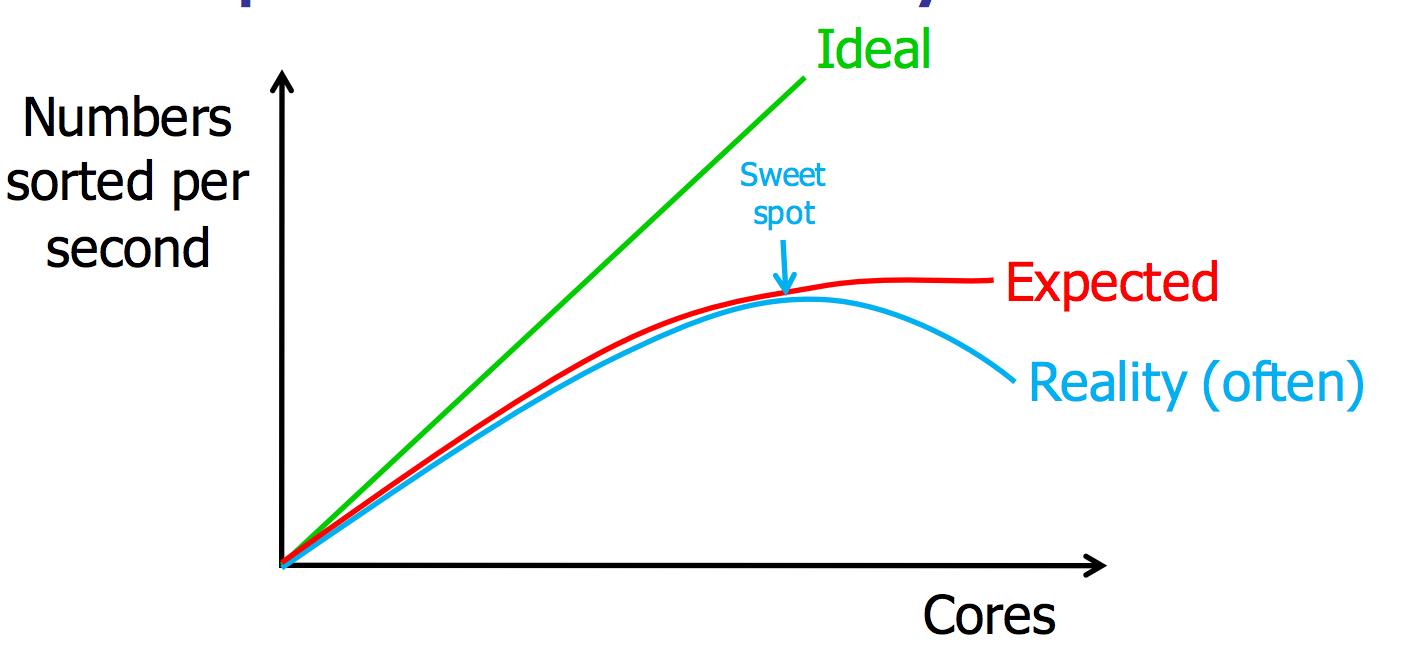
\includegraphics[width=\linewidth]{parall.png}

This graphic shows the Amdahl's law which gives the theoretical speedup in latency of the execution of a task at fixed workload that can be expected of a system whose resources are improved. It depends from parallelizable portion of the program.

\subsubsection{Coarse-grain vs. fine-grain parallelism}

Coarse-grain (gros grain) is better, less coordination messages (less overhead).


\subsubsection{Dependencies}

Dependencies : if tasks depend on other tasks => Limits the degree of parallelism. Minimum completion time (and thus maximum speedup) is determined by the longest path from start to finish. 

\subsubsection{Heterogeneity}

Heterogeneity : if tasks are harder than others or not all cores are equally fast. => Result: Scheduling problem (can be hard to solve).

\subsection{Parallelism vs Concurrency}

Parallelism refers to techniques to make programs faster by performing several computations in parallel (multi-core processors, compute clusters)

Concurrency is the composition of independently executing computations (It is a way to structure software and make it more usable)

\subsubsection{Race condition}

Result of the computation depends on the exact timing of the two threads of execution, i.e., the order in which the instructions are executed. Concurrent updates to the same state. 

\subsubsection{Goal: Consistency}

\begin{description}
\item[Sequential consistency] The result of any execution is the same as if the operations of all the cores had been executed in some sequential order, and the operations of each individual processor appear in this sequence in the order specified by the program.

\item[Strong consistency] After update completes, all subsequent accesses will return the updated value.

\item[Weak consistency] After update completes, accesses do not necessarily return the updated value; some condition must be satisfied first

\item[Eventual consistency] Specific form of weak consistency: If no more updates are made to an object, then eventually all reads will return the latest value

\item[Eventual consistency: Causal consistency] If client A has communicated to client B that it has updated a data item, a subsequent access by B will return the updated value, and a write is guaranteed to supersede the earlier write. Client C that has no causal relationship to client A is subject to the normal eventual consistency rules.

\item[Eventual consistency: Read-your-writes consistency] Client A, after it has updated a data item, always accesses the updated value and will never see an older value.

\item[Eventual consistency: Session consistency] Like previous case but in the context of a session, for as long as the sessions remains alive.

\item[Eventual consistency: Monotonic read consistency] If client A has has seen a particular value for the object, any subsequent accesses will never return any previous values.

\item[Eventual consistency: Monotonic write consistency] In this case the system guarantees to serialize the writes by the same process. Systems that do not guarantee this level of consistency are notoriously hard to program.

\item[Few consistency properties can be combined] monotonic reads + read-your-writes most desirable for eventual consistency.
\end{description}

\subsection{Architectures}
\subsubsection{Symmetric Multiprocessing (SMP)}
All processors share the same memory. Any CPU can access any byte; latency is always the same. Pros: Simplicity, easy load balancing. Cons: Limited scalability (~12 processors), expensive.

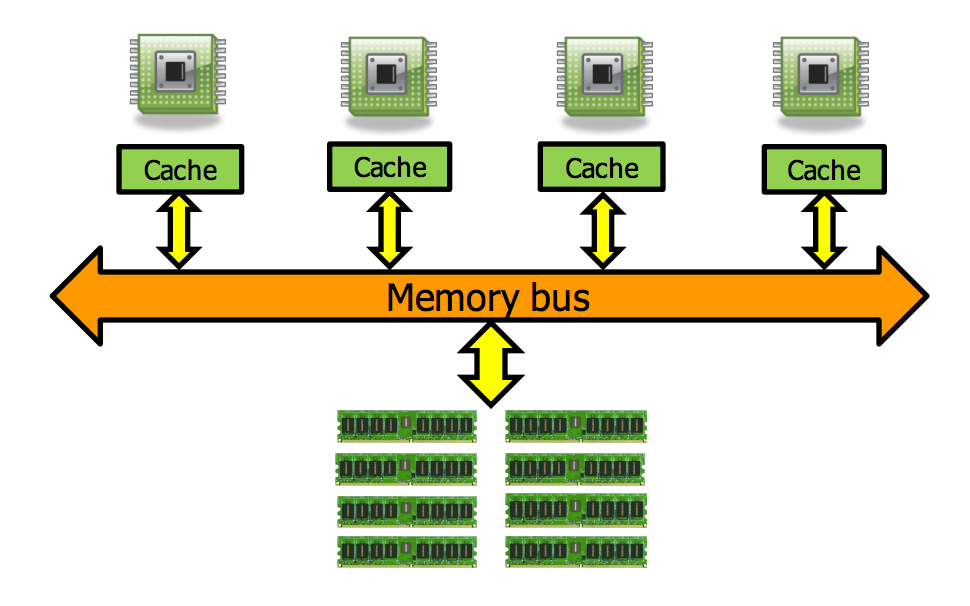
\includegraphics[width=\linewidth]{smp.png}

\subsubsection{Non-Uniform Memory Architecture (NUMA)}
Memory is local to a specific processor. Each CPU can still access any byte, but accesses to 'local' memory are considerably faster (2-3x). Pros: Better scalability. Cons: Complicates programming a bit, scalability still limited. 

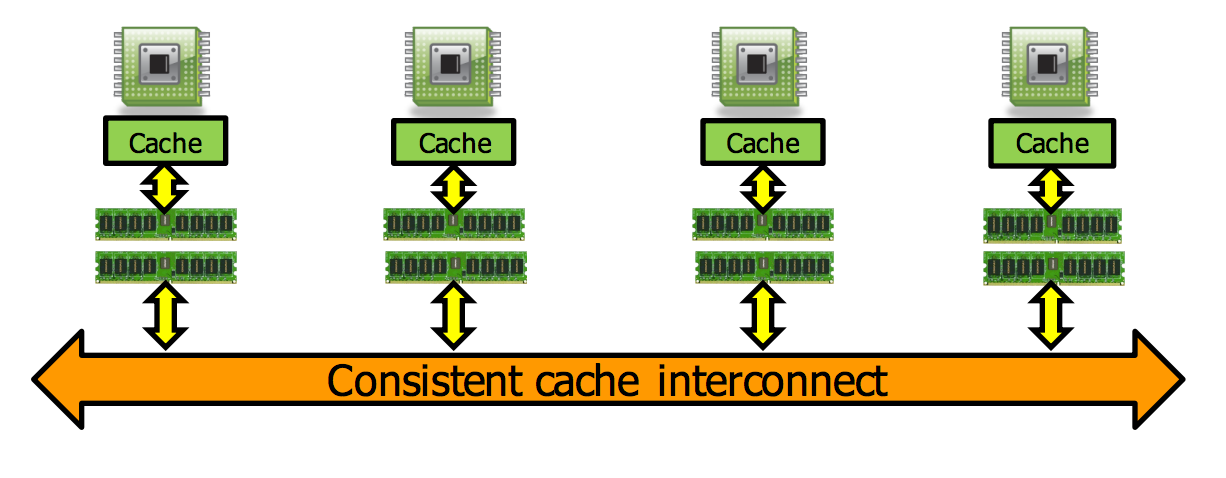
\includegraphics[width=\linewidth]{numa.png}

\subsubsection{Shared-Nothing}

Independent machines connected by network. Each CPU can only access its local memory; if it needs data from a remote machine, it must send a message there. Pros: Much better scalability. Cons: Requires a different programming model. 

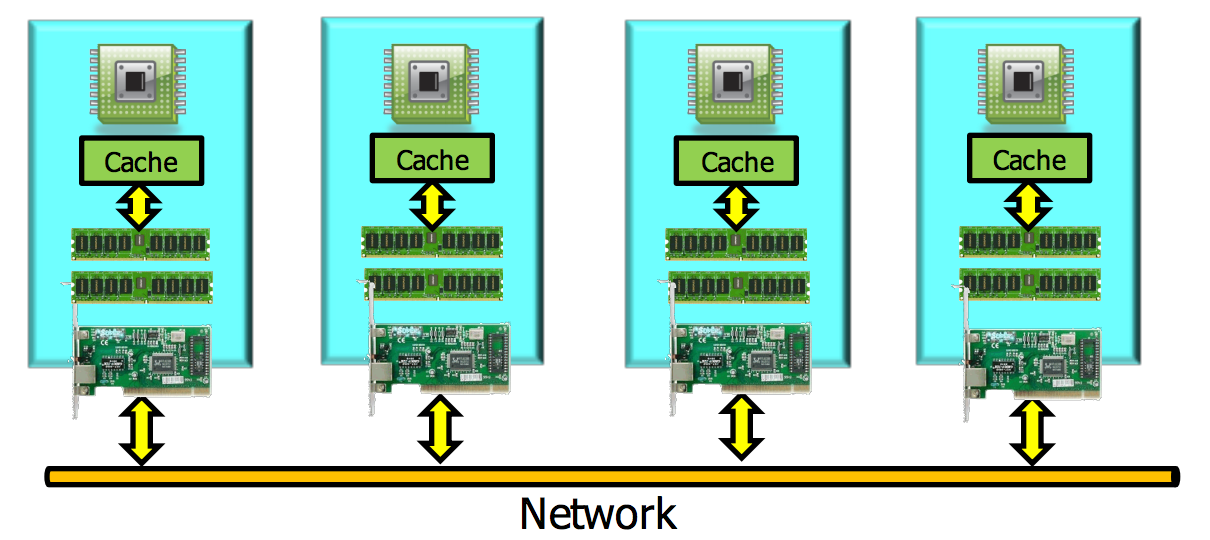
\includegraphics[width=\linewidth]{shared-nothing.png}

Wide area network : RTT (Round Trip Time) matters.. a lot !

\subsection{Fault and failure in distributed systems}

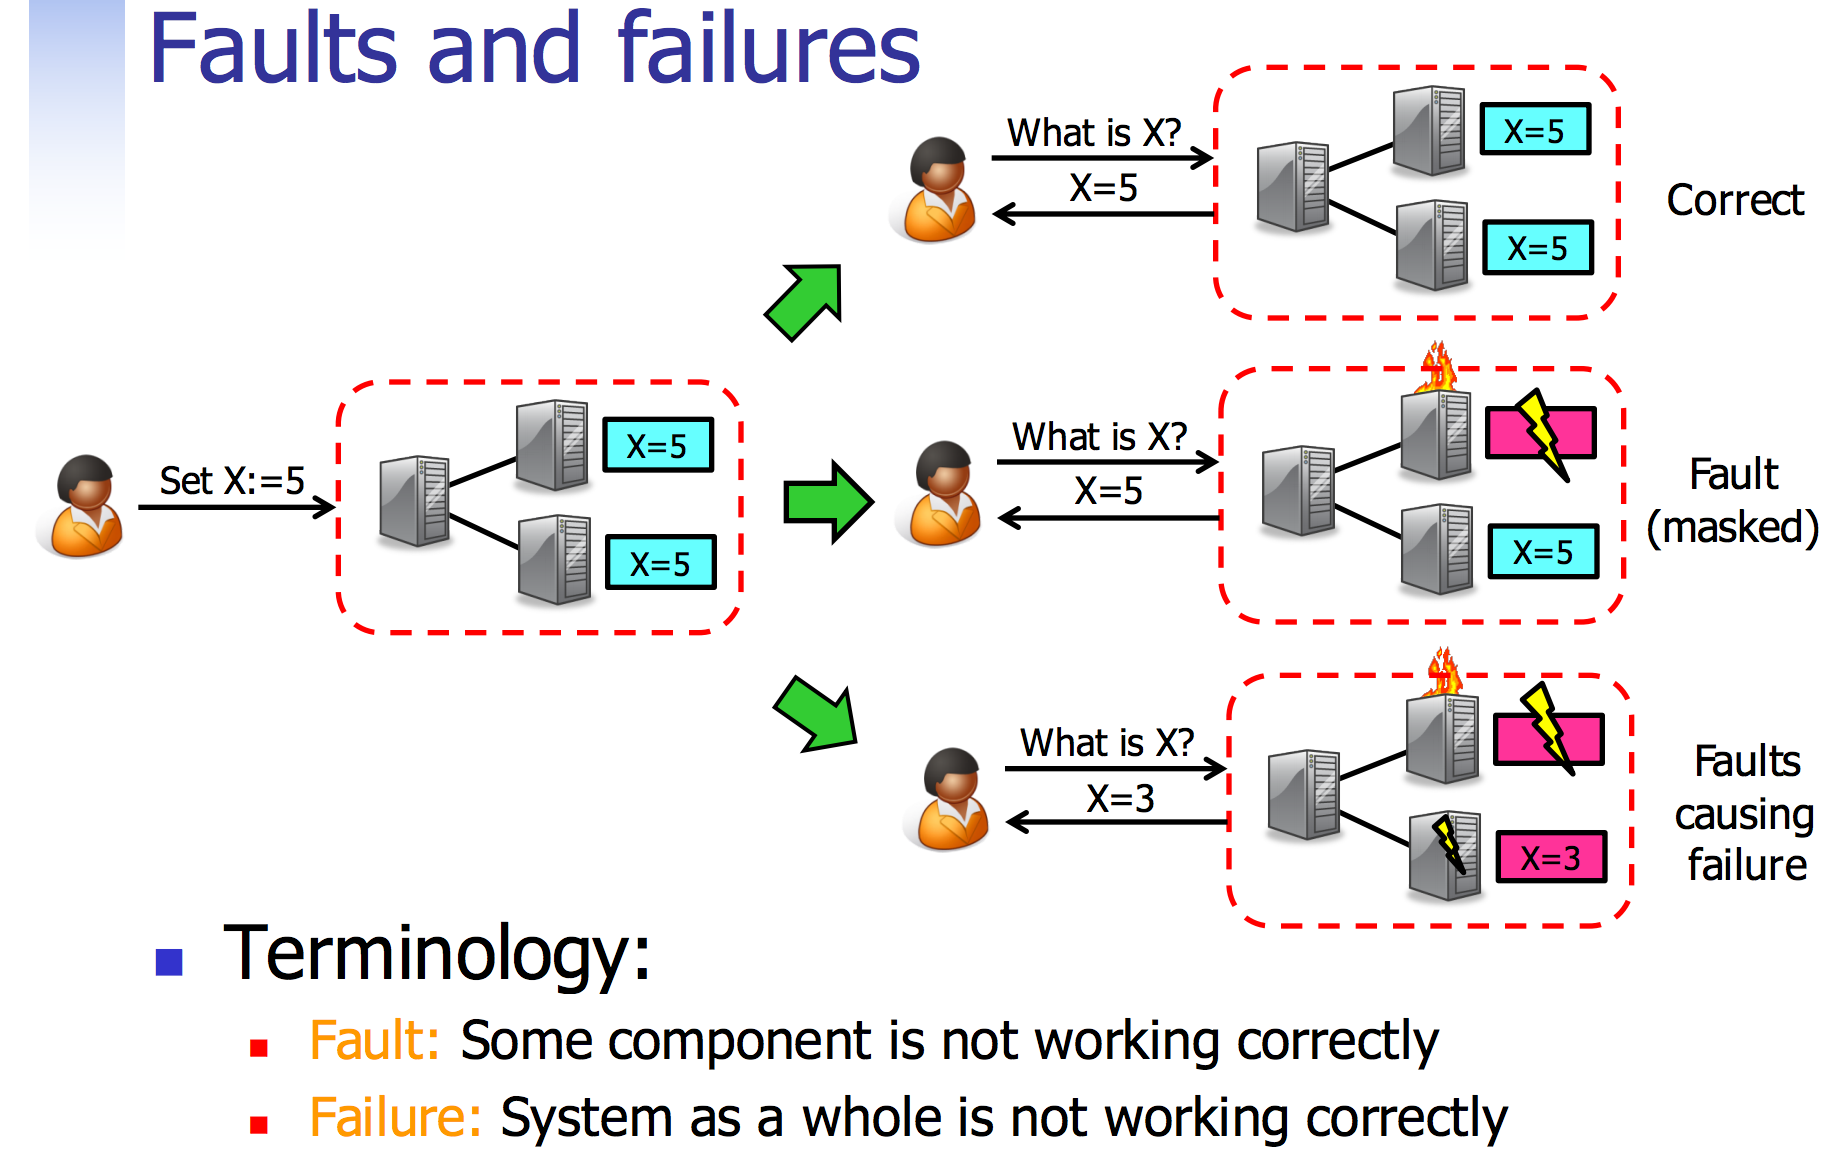
\includegraphics[width=\linewidth]{fault-fail.png}

Type of faults:
\begin{description}
\item[Crash faults] Node simply stop (OS crash, power loss)
\item[Rational behavior] Owner manipulates node to increase profit (Traffic attraction attack)
\item[Byzantine faults] Arbitrary - faulty node could do anything  (Node compromised by a hacker, compromised data, etc.)
\end{description}

A fault can lead to a domino efffect. Fault can be correlated with others.

What can be done ?
\begin{description}
\item[Prevention and avoidance]  Temporal Logic Action (formal methods are a particular kind of mathematically based techniques for the specification, development and verification of software and hardware systems)
\item[Detection] Cross-check network's route announcements with other information to see whether it is lying, and hold it accountable if it is
\item[Masking]  Store replicas of the data on multiple nodes; if data is lost or corrupted on one of them, we still have the other copies. Problem => Consistency (see before)
\item[Mitigation] 
\end{description}

\subsection{Storage system consistency: example}

We have N nodes that can store data.
To write a value: Pick W replicas and write the value to each, using a fresh timestamp
To read a value:
\begin{itemize}
\item Pick R replicas and read the value from each
\item Return the value with the highest timestamp
\item If any replicas had a lower timestamp, send them the newer value
\end{itemize}

Strong consistency :
\begin{description}
\item[Majority quorum] Always write to and read from a majority of nodes. At least one node knows the most recent value.  tolerate up to ⌈N/2⌉ - 1 crashes. But have to read/write ⌊N/2⌋ + 1 values.
\item[Read/write quorums] Read R nodes, write W nodes, s.t. R + W > N. Adjust performance of reads/writes. But availability can suffer.
\item[Consensus solutions] Paxos (for crash faults), PBFT (for Byzantine faults). Idea : Correct replicas ``outvote'' faulty ones.
\end{description}
 
The cap theorem : We can get at most two out of the three
\begin{itemize}
\item Consistency : All clients single up-to-data copy of the data, even in the presence of concurrent updates
\item Availability: Every request (including updates) received by a non-failing node in the system must result in a response, even when faults occur
\item Partition-tolerance: Consistency and availability hold even when the network partitions
\end{itemize}

Dealing with network partitions when a partition is cut : Enter an explicit partition mode that can limit some operations.


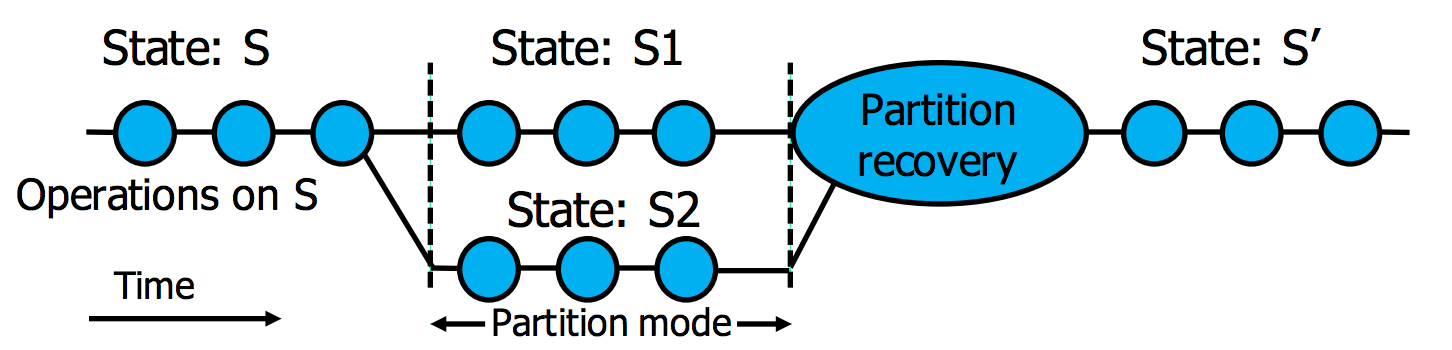
\includegraphics[width=\linewidth]{part.png}

\subsection{Relaxed consistency: ACID vs. BASE}

ACID => Atomicity, Consistency, Isolation, Durability
BASE => Basically Available, Soft-state, Eventually consistent

\subsubsection{Consistency and partitions}
=> Use replication to mask limited \# of faults
=> Partition tolerance, availability, consistency? Typically trade-off between C and A

\section{Another chapter}


\end{document}
